\section{Evaluation}

\begin{itemize}
  \item User testing
  \item Client feedback
\end{itemize}


\subsection{Market Readiness}

The Choona prototype has proved that the idea itself works as a technical system and is well received by users, however there are still several important milestones to complete before Choona is be ready to release to the general public.

\begin{itemize}
  \item \textbf{Audio Licensing and Partnerships}\\
    We've previously discussed the issues surrounding music licensing for public locations and how they can be resolved, however another hurdle that will have to be tackled is the restrictions that many audio sources have in their terms of service. Spotify, for example, has a blanket ban on using their service in any commercial or non-personal environment\footcite{spotifypublic} with the exception of official partnership agreements\footcite{spotifypartners}. This is most likely going to be the case for most, if not all, online music services, meaning we will have to approach each company on a case-by-case basis with a partnership proposal. On the surface this may just seem like a business development issue, however it could also have an impact on Choona's software as well. For example, Spotify might require their own logo and advertising to be embedded in the app which will require additional development work and integration with third party systems.

    There is also a possibility that rival music services would not be happy with Choona supporting them both; it is highly unlikely that Spotify will endorse and enter a partnership agreement with a product that is also in a partnership with Google Music, especially if the product is still in the prototype stages. Therefore in order to get to get to market in a reasonable time frame it may be necessary to focus on partnering with one or two main services initially.

  \item \textbf{Client Management Interface}
    Choona currently has no management systems or interfaces for clients to manage their accounts. We plan to implement a separate mobile application and access API called Fishtank, designed purely for use by clients and not the general public. It is becoming increasingly common for large multi-context applications to break their apps down into multiple single-context apps; Facebook's release of their separate Pages Manager\footcite{facebookpages} is an excellent example. Having separate applications helps to keep code bases leaner and allows you to update more frequently with less chance of breaking other functionality.

    Fishtank will offer a wide range of management options to clients:
    \begin{itemize}
      \item \textit{Geofence manipulation}: designation of geofences at verified Choona locations
      \item \textit{User management}: ability to ban users, give them rewards etc.
      \item \textit{Playlist settings}: configure default playlists to load when the user-managed queue is empty, restrict searching to only pull from a subset of available tracks, define content restrictions on available songs (such as explicit content exclusion), select different upvote/downvote algorithms to use
      \item \textit{Playlist override}: ability to skip songs on the fly, pause the entire stream, bump a song to the top of the queue
      \item \textit{Ad/offer management}: insertion of visual adverts into various placeholders of the Choona application (e.g. playlist banner), creating and integrating audio adverts into the Choona stream, target offers and adverts to specific subsets of users (e.g. give frequent users a discount)
      \item \textit{Speaker adapter settings}: control the output volume, select different geolocations
    \end{itemize}

    Without Fishtank it will be hard to appeal to enterprise clients that will be looking for a polished, well-rounded system that is easy to set up and control.

  \item \textbf{User accounts}
    We currently do not maintain any server-side data about users. This means it is impossible to store long-term data such as listening history or user access levels. In order to make this happen a database service needs to be created that will be responsbile for storing account data. This will be accessible via a dedicated user service that is responsible for combining profile data from Auth0 with context-specific data from the Choona user database, as shown in figure \ref{fig:user-service}.

    \begin{figure}[h!]
      \centering
      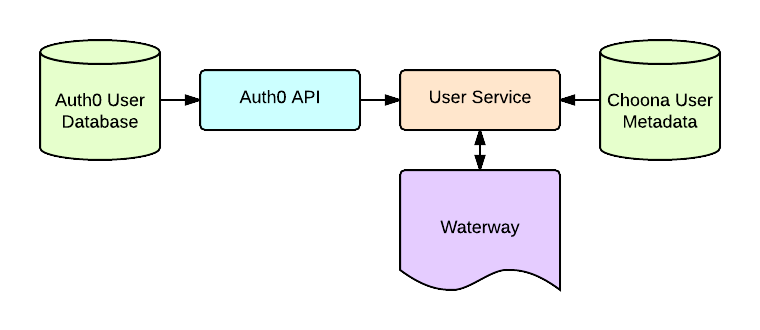
\includegraphics[width=0.8\textwidth]{./img/userservice.png}
      \caption{Future user service}
      \label{fig:user-service}
    \end{figure}

  \item \textbf{Infrastructure improvements and testing}
    The majority of the code used in the prototype is not currently covered by unit tests, making it unsafe for proper production use. Every service in the Choona infrastructure needs to have 100\% code coverage before being officially released. Furthermore every aspect of the system needs to be stress tested to ensure it is capable of supporting a high number of users. This will most likely require load balancing of certain resource-intensive services such as the Socket.IO API and the Spotify source that directly interface and manipulate audio data.
\end{itemize}